\chapter{Minimalbeispiel 3D-Stereokalibrierung und Szenenrekonstruktion bei Kameras gleicher Auflösung}



\section{Vorgehen: Projektion eines Quaders in zwei verschieden transformierte Kameras}

Um den Mathematischen Vorgang der stereoskopischen Szenenrekonstruktion zu verdeutlichen, wurde ein Minimalszenario erstellt. Für dieses Minimalszenario wurde ein Objekt in diesem Falle ein Quader in ein zuvor Definiertes Weltkoordinatensystem gesetzt. Des Weiteren wurden zwei Kameras in die Szene platziert. Kamera 1 ist von der Lage Deckungsgleich mit dem Weltkoordinatensystem. Kamera 2 wurde verschoben und Rotiert, um so ein anderes Abbild des Objekts auf dem Sensor so produzieren. Für unsere Berechnungen der Szene sind äußere und innere Kameraparameter von uns festgelegt worde. Für eine Szenenrekonstruktion mit realen Bedinungen müssen diese zunächst ermittelt werden, um die aufgezeigten mathematischen Vorgänge anwenden zu können.\\

	Für die Stereokamerakalibrierung wird eine der beiden Kameras relativ zur ersten Kamera um einen Vector \ensuremath{\vec{v}} verschoben und anschließend um einen Winkel \ensuremath{\alpha} um die e2 Achse (vgl. mit Dokumentation Koordinatensysteme) gedreht. 
Für die Rotation um \ensuremath{e_2} gilt folgende Drehmatrix:

\begin{gather}		
R= 
\begin{pmatrix}
\cos(\alpha)&0&\sin(\alpha)\\
0&1&0\\
-\sin(\alpha)&0&\cos(\alpha)
\end{pmatrix}
\end{gather}

Um die Transformationsmatrix \ensuremath{M} welche die Rotation und die Translation beinhaltet zu bekommen werden \ensuremath{R} und \ensuremath{\vec{v}} miteinander verrechnet, hierzu wird aus \ensuremath{\vec{v}} eine Matrix \ensuremath{V} gebildet. 

\begin{gather}
V= 
\begin{pmatrix}
1&0&0&-v_1\\
0&1&0&-v_2\\
0&0&1&-v_3			
\end{pmatrix}\\
M=R^T\cdot V\\
M=		\begin{pmatrix}
\cos(\alpha)&0&-\sin(\alpha)\\
0&1&0\\
\sin(\alpha)&0&\cos(\alpha)
\end{pmatrix} 
\cdot
\begin{pmatrix}
1&0&0&-v_1\\
0&1&0&-v_2\\
0&0&1&-v_3			
\end{pmatrix}\\
M=
\begin{pmatrix}
\cos(\alpha)&0&-\sin(\alpha)&-v_1\cos(\alpha)+v_3\sin(\alpha)\\
0&1&0&-v_2\\
\sin(\alpha)&0&\cos(\alpha)&-v_1\sin(\alpha)-v_3\cos(\alpha)\\
\end{pmatrix}
\end{gather}\\

Die entstandene Matrix \ensuremath{M} beschreibt die Transformation der der Kamera 2 und somit auch die Transformation des Koordinatensystems der Kamera 1 in das Koordinatensystem der Kamera 2.

\begin{minipage}{\linewidth}
	\centering
	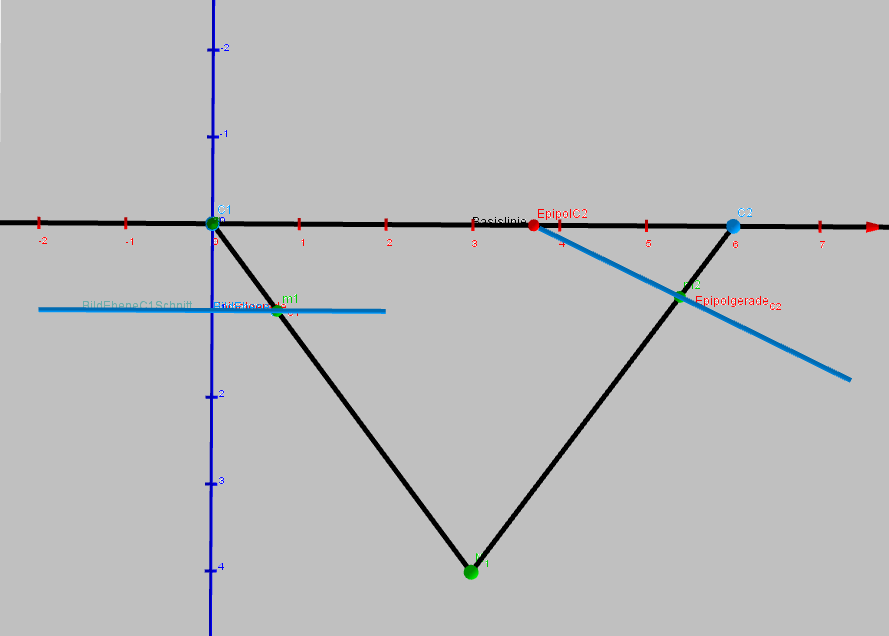
\includegraphics[width=1.\linewidth]{images/TopDownSystem.png}
	\captionof{figure}{Top-Down-Ansicht des entstandenen Aufbaus der Kameras}
\end{minipage}\\ \\

\begin{minipage}{\linewidth}
	\centering
	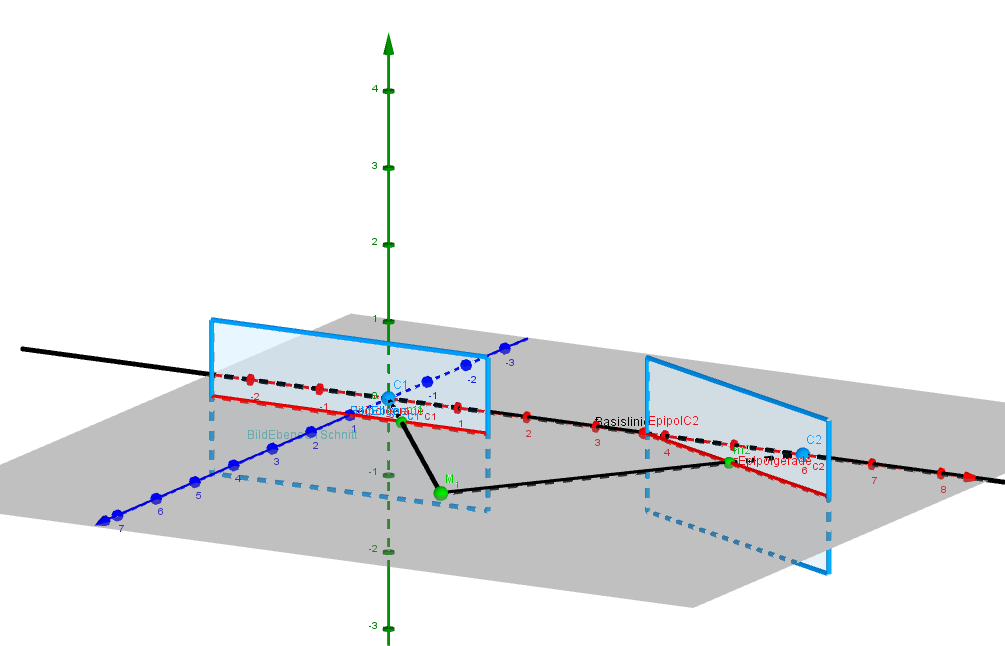
\includegraphics[width=1.\linewidth]{images/3DAnsichSystem.png}
	\captionof{figure}{3D-Ansicht des entstandenen Aufbaus der Kameras}
\end{minipage}\\ \\

%	\subsubsection{Drehung um einen Drehpunkt}	
%	Funktion RotationOfCameraAroundPivotPoint 

\section{Berechnung der Projetkionsmatritzen}

Die Punkte \ensuremath{a,b,c,d,a',b',c',d',d2} in Weltkoordinaten sind bekannt. Die ersten acht Punkte bilden gemeinsam einen Quader, der neunte Punkt ist aus diesem Quader ausgelagert.	
Um die Koordinaten der Punkte in Kamera 1 und Kamera 2 Koordinaten zu Transformieren, muss zusätzlich zur Transformationsmatrix für Kamera2 noch die Abbildungsmatrix \ensuremath{AB1} und \ensuremath{AB2} der jeweiligen Kamera berücksichtigt werden. 

\begin{gather}		
AB1 =
\begin{bmatrix}
\zeta_{K1}&0&0&0\\
0&\zeta_{K1}&0&0\\
0&0&\zeta_{K1}&0\\
0&0&1&0
\end{bmatrix}\\
AB2 =
\begin{bmatrix}
\zeta_{K2}&0&0&0\\
0&\zeta_{K2}&0&0\\
0&0&\zeta_{K2}&0\\
0&0&1&0
\end{bmatrix}
\end{gather}

Um die Projektionsmatrizen \ensuremath{PM1} und \ensuremath{PM2} zu berechnen, bekommt die Matrix \ensuremath{M} noch eine Homogene erweiterung und sieht dann folgendermaßen aus:

\begin{gather}
M=
\begin{bmatrix}
\cos(\alpha)&0&-\sin(\alpha)&-v_1\cos(\alpha)+v_3\sin(\alpha)\\
0&1&0&-v_2\\
\sin(\alpha)&0&\cos(\alpha)&-v_1\sin(\alpha)-v_3\cos(\alpha)\\
0&0&0&1
\end{bmatrix}\\
PM1 = AB1\cdot I_{4x4} \\
PM1 =
\begin{bmatrix}
\zeta_{K1}&0&0&0\\
0&\zeta_{K1}&0&0\\
0&0&\zeta_{K1}&0\\
0&0&1&0
\end{bmatrix}
\end{gather}
\ensuremath{I} ist die Einheitsmatrix, wir gehen davon aus das Kamera 1 weder eine Drehung noch eine Translation beinhaltet und ihr Ursprung sich im Weltkoordinatenurspung befindet.\\


\begin{gather}
PM2 = AB2 \cdot M\\
PM2 =
\begin{bmatrix}
\zeta_{K2} \cos(\alpha)&0&\zeta_{K2} \sin(\alpha)&-\zeta_{K2} (v_1\cos(\alpha)+v_3\sin(\alpha) )&0\\
0&1&0&\zeta_{K2}-v_2&0\\
\zeta_{K2}\sin(\alpha)&0&\zeta_{K2}\cos(\alpha)&-\zeta_{K2}(v_1\sin(\alpha)+v_3\cos(\alpha))\\
0&0&0&0&1
\end{bmatrix}
\end{gather}

\section{Transformation der Weltpunkte in Koordinaten der Koordinatensysteme von beiden Kameras}

	Die 3D-Punkte \ensuremath{a,b,c,d,a',b',c',d',d2}, werden um eine Homogene Komponenten erweitert und mit den Projektionsmatrizen \ensuremath{PM1} und \ensuremath{PM2} verrechnet. Die so neu entstehenden Punktematrix \ensuremath{PK1} mit  \ensuremath{K1a,K1b,K1c,K1d,K1a',K1b',K1c',K1d',K1d2} und \ensuremath{PK2} mit \ensuremath{K2a,K2b,K2c,K2d,\linebreak K2a',K2b',K2c',K2d',K2d2} beschreiben jeweils den selben Quader aus den beiden verschiedenen Kamerakoordinatensystemen.\\

\begin{gather}		
PK1 =		
\begin{bmatrix}
\begin{pmatrix}
\\a\\\\1
\end{pmatrix}&
\begin{pmatrix}
\\b\\\\1
\end{pmatrix}&
\begin{pmatrix}
\\c\\\\1
\end{pmatrix}&
\begin{pmatrix}
\\d\\\\1
\end{pmatrix}&
\begin{pmatrix}
\\a'\\\\1
\end{pmatrix}&
\begin{pmatrix}
\\b'\\\\1
\end{pmatrix}&
\begin{pmatrix}
\\c'\\\\1
\end{pmatrix}&
\begin{pmatrix}
\\d'\\\\1
\end{pmatrix}&
\begin{pmatrix}
\\d2\\\\1
\end{pmatrix}
\end{bmatrix}
\cdot
PM1\\
PK2 =		
\begin{bmatrix}
\begin{pmatrix}
\\a\\\\1
\end{pmatrix}&
\begin{pmatrix}
\\b\\\\1
\end{pmatrix}&
\begin{pmatrix}
\\c\\\\1
\end{pmatrix}&
\begin{pmatrix}
\\d\\\\1
\end{pmatrix}&
\begin{pmatrix}
\\a'\\\\1
\end{pmatrix}&
\begin{pmatrix}
\\b'\\\\1
\end{pmatrix}&
\begin{pmatrix}
\\c'\\\\1
\end{pmatrix}&
\begin{pmatrix}
\\d'\\\\1
\end{pmatrix}&
\begin{pmatrix}
\\d2\\\\1
\end{pmatrix}
\end{bmatrix}
\cdot
PM2
\end{gather}

Die entstanden Koordinaten sehen dann entsprechen Gleichung 16 aus und müssen dann wieder auf eine homogene Form gebracht werden. 

\begin{gather}
aK2 = 
\begin{pmatrix}
x\\y\\\delta z\\\delta
\end{pmatrix}
\leadsto aK2= 
\begin{pmatrix}
\frac{x}{\delta}\\ \frac{y}{\delta}\\ \frac{\delta z}{\delta}\\ \frac{\delta}{\delta}
\end{pmatrix}
\leadsto aK2 =
\begin{pmatrix}
\tilde{x}\\
\tilde{y}\\
z\\
1
\end{pmatrix}
\end{gather}\\

\begin{minipage}{\linewidth}
	\centering
	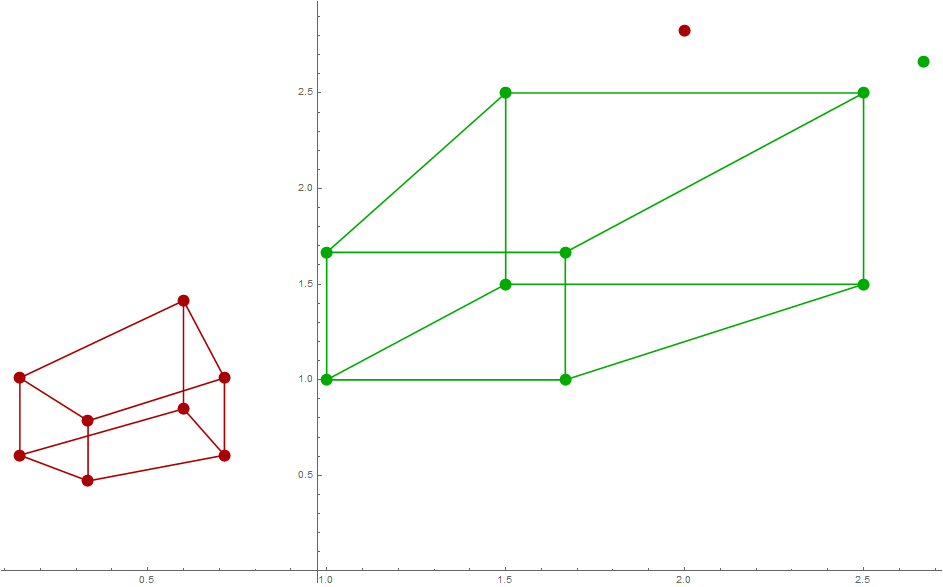
\includegraphics[width=0.8\linewidth]{images/Camer1and2Objects.png}
	\captionof{figure}{Grün zeigt den Quader aus sicht von Kamera 1. Das größere Quadrat sind die vorderen Punkte \ensuremath{a,b,c,d}, das kleinere Quadrat sind die hinteren Punkte \ensuremath{a',b',c',d'}. Rot zeigt denselben Quader aus Sicht vom Kamera 2, wenn diese in +\ensuremath{e_1}-Richtung verschoben und um 45° um \ensuremath{e_2} gedreht wurde}
\end{minipage}\\
\section{Berechnung der projizietrten Punkte auf den beiden Bildebenen}

Um die 3D-Kamerakoordinaten auf die 2D-Bildebene zu Projizieren muss man lediglich die Tiefeninformation der Punkte \ensuremath{PK1} und \ensuremath{PK2} entnehmen und durch die homogene Koordinate ersetzen. Die folgende Gleichung zeigt ein Beispiel dazu 

\begin{gather}
aK2 =
\begin{pmatrix}
\tilde{x}\\
\tilde{y}\\
z\\
1
\end{pmatrix} 
\leadsto aBK2 = 		
\begin{pmatrix}
\tilde{x}\\
\tilde{y}\\
1
\end{pmatrix}
\end{gather}

\section{Umrechnung von Bildebenenkoordinaten in Sensorkoordinaten}
	Für die Umrechnung der Bildebenenkoordinaten \ensuremath{BK1} und \ensuremath{BK2} in Sensorkoordianten, muss der sogenannte Pixelpitch des Sensors bekannt sein. Nehmen wir für unser Beispiel man an wir haben einen PixelPitch von 1. Dann bedeutet dies, dass die Bilebenenkoordinaten in mm 1:1 in die Sensorkoordinaten in Pixel umgesetzt werden können. In der Realität ist dies aber eher selten der Fall. \\
Das Sensorkoordinatensystem wird folgendermaßen beschrieben:

\begin{gather}
K_s = (\vec{u},\vec{v},O_s)\\	
\vec{u} = u_1b_1+u_2b_2\\
\vec{v} = v_1b_1+v_2b_2\\
O_s = O_B+p_1b_1+p_2b_2\\
(\vec{u},\vec{v},O_s)=(b_1,b_2,O_B)\cdot
\begin{bmatrix}
u_1&u_2&p_1\\
v_1&v_2&p_2\\
0&0&1
\end{bmatrix}	\\
M_S = 	
\begin{bmatrix}
u_1&u_2\\
v_1&v_2
\end{bmatrix}
\end{gather}

Stellen wir nun \ensuremath{	\leftidx{_{K_{s}}}{\begin{bmatrix}
			\pi
	\end{bmatrix}}{_{K_{}}}} dar\\

\begin{gather}
\begin{bmatrix}
&&\\
&M^{-1}& -M\begin{pmatrix}p_1\\p_2\end{pmatrix}^{-1}\\
&&\\
0&0&1
\end{bmatrix}
\cdot
\begin{bmatrix}
-\zeta&0&0&0\\
0&-\zeta&0&0\\
0&0&1&0
\end{bmatrix}
=
\begin{bmatrix}
&&&0\\
&-\zeta M^{-1}& -M\begin{pmatrix}p_1\\p_2\end{pmatrix}^{-1}&0\\
&&&\\
0&0&1&0
\end{bmatrix}\\
aSK2 = 
\begin{bmatrix}
&&&0\\
&-\zeta M^{-1}& -M\begin{pmatrix}p_1\\p_2\end{pmatrix}^{-1}&0\\
&&&\\
0&0&1&0
\end{bmatrix} 
\cdot
aBK2
\end{gather}\\

Als Beispiel nehmen wir an wir haben einen Pixelpitch \ensuremath{p} und es gilt \ensuremath{\vec{u} = 1pb_1} und \ensuremath{\vec{v}=2pb_2}. Des Weiteren sei \ensuremath{p_1} =15 und \ensuremath{p_2} = 20.

\begin{gather}
O_s = O_B - \vec{u}-\vec{v} \leadsto O_s = O_B-15b_1-20b_2\\
M_S = \begin{bmatrix}
1&0\\
0&2
\end{bmatrix} \leadsto M^{-1} =
\begin{bmatrix}
\frac{1}{p}&0\\
0&\frac{1}{2p}
\end{bmatrix}\\
\leadsto [\pi]=
\begin{bmatrix}
\frac{\zeta}{p}&0&15&0\\
0&\frac{\zeta}{2p}&20&0\\
0&0&1&0
\end{bmatrix}\\
\end{gather} 



\section{Ermitteln der Fundamentalmatrix mit Hilfe des 8-Point-Algorithms}
	Sind die Sensorkoordinaten berechnet, kann nun die Fundamentalmatrix mit Hilfe des 8-Point-Algorithms ermittelt werden. Für die Fundamentalmatrix benötigen wir mindestens sieben Punktekorrespondenzen. Mit sieben Punkten bekommen wir als Lösung des 8-Point-Algorithm zwei linear unabhängige Kerne als Lösung der Koeffizientenmatrix mit welchen weiter verfahren werden muss (Mehr dazu später). Hartley und Zisserman schlagen vor, dass sich zur Sicherheit am besten neun Punkte eigenen. Zu beachten ist nämlich, dass wenn die Punkte in sofern voneinander abhängen, dass immer 2 Punkte auf der selben Epipolarlinie liegen, verliert unsere Koeffizientenmatrix an Rang und wir bekommen  wie bei den sieben Punkten zwei Lösungen für den Kern. Aufgrund dessen haben wir einen neunten Punkt\ensuremath{d2} zu unserem Quader hinzugefügt, welcher nicht Gefahr läuft auf der selben Epipolarlinien wie ein anderer Punkt zu liegen.\\

Wir haben also nun unsere 9 Punkte auf dem Sensor der Kamera 1 \ensuremath{SK1} und dem Sensor der Kamera 2 \ensuremath{SK2}. Die Fundamentalmatrix ist definiert als

\begin{gather}
x'^T F x =0
\end{gather}

Die Fundamentalmatrix ist eine 3x3-Matrix mit Rang 2. Um sie zu ermitteln muss zunächst eine Koeffizientenmatrix nach folgendem Schema erstellt werden: 

\begin{gather}
F=\begin{bmatrix}
f_{11}&f_{122}&f_{13}\\
f_{21}&f_{22}&f_{23}\\
f_{31}&f_{32}&f_{33}
\end{bmatrix}\\
\begin{bmatrix}
x'_n&y'_n&1
\end{bmatrix} 
\cdot
\begin{bmatrix}
f_{11}&f_{122}&f_{13}\\
f_{21}&f_{22}&f_{23}\\
f_{31}&f_{32}&f_{33}
\end{bmatrix}
\cdot
\begin{bmatrix}
x_n\\y_n\\1
\end{bmatrix} =0\\
f_{11}x_nx'_n+f_{12}y_nx'_n+f_{13}x'_n+f_{21}x_ny'_n+f_{22}y_ny'_n+f{23}y'_n+f_{31}x_n+f_{32}y_n+f_{33} =0\\
(x_nx'_n,y_nx'_n,x'_n,x_ny'_n,y_ny'_n,y'_n,x_n,y_n,1)\cdot f =0\\
\begin{bmatrix}
x_1x'_1&y_1x'_1&x'_1&x_1y'_1&y_1y'_1&y'_1&x_1&y_1&1\\
x_2x'_2&y_2x'_2&x'_2&x_2y'_2&y_2y'_2&y'_2&x_2&y_2&1\\
.&.&.&.&.&.&.&.&.\\
.&.&.&.&.&.&.&.&.\\
.&.&.&.&.&.&.&.&.\\
x_nx'_n&y_nx'_n&x'_n&x_ny'_n&y_ny'_n&y'_n&x_n&y_n&1
\end{bmatrix}
\cdot 
\begin{pmatrix}
f_{11}\\f_{12}\\f_{13}\\f_{21}\\f_{22}\\f_{23}\\f_{31}\\f_{32}\\f_{33}
\end{pmatrix}
= 0
\end{gather}

Der Kern und alle seine Vielfache sind Lösungen für die Fundamentalmatrix. Um den Kern aus der Koeffizientenmatrix zu berechnen wird der null-space oder auch Nullraum ermittelt. der null-space beschreibt denjenigen Vektor, welcher durch multiplizieren mit der Koeffizientenmatrix gleich den Nullvektor ergibt.

\begin{gather}
A\cdot f 
\end{gather} \\

Also Kern bekommt man in diesem Fall eine Liste mit Einträgen. 
Diese neun Einträge ergeben dann die Werte der 3x3-Fundamentalmatrix. 


\section{Berechnen der Epipole und Epipolargeraden mit der Fundamentalmatrix}
	Mit Hilfe der Fundamentalmatrix und dem Wissen über die Epipolargerometrie, kann man die Epipole \ensuremath{e} und \ensuremath{e'}, sowie die Epilolargeraden \ensuremath{l} und \ensuremath{l'} ermitteln. Im ersten Abschnitt wird die ermittlung mit Hilfe der Fundamentalmatrix aufgezeigt und in Kapitel 1.2.1 wird nochmal drauf eingegangen und aufgezeigt, wie sich die Epipolarlinien und Epipole geometrisch Konstruieren lassen.\\

Mit der Fundamentalmatrix lassen sich die Epipolargerade folgendermaßen berechnen

\begin{gather}
l' = F \cdot x\\
l = F^T \cdot x'
\end{gather}\\

\ensuremath{l'} ist die zu \ensuremath{x} korrespondierende Epipolargerade. \ensuremath{l} ist die zu \ensuremath{x'} korrespondierende Epipolargerade. Zu Berechnung des Epipols \ensuremath{e} muss der Rechte Null-Space von F ermitteln werden und für den Epipol \ensuremath{e'} brauchen wir den linken Null-Space. Um diesen zu bekommen ermitteln wir wie bekannt den Kern aber diesmal von \ensuremath{F^T} statt \ensuremath{F}. Die Abbiludng 4 zeigt, dass Ergebnis.

\begin{minipage}{\linewidth}
	\centering
	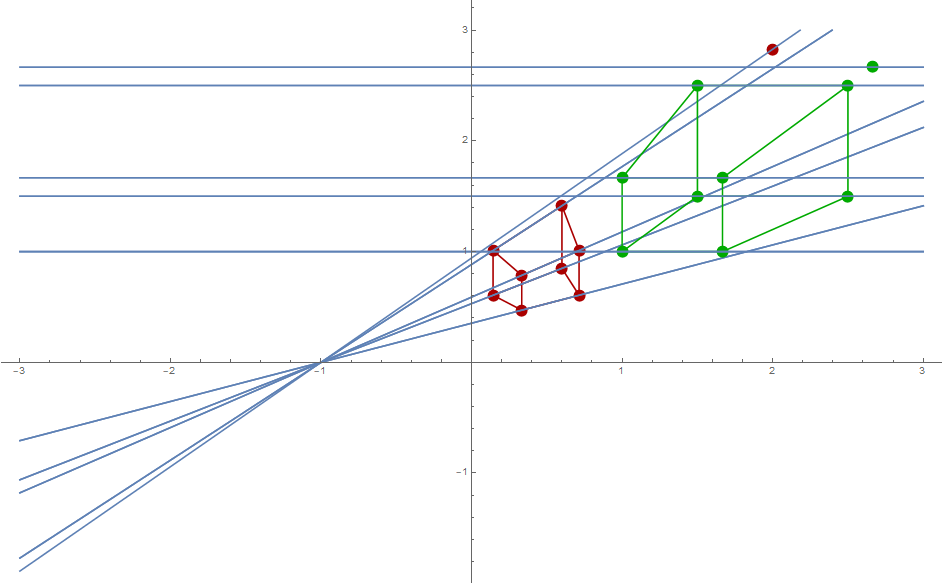
\includegraphics[width=1.\linewidth]{images/Epipole_Epipollinien.png}
	\captionof{figure}{Die blauen Geraden zeigen die jeweiligen Epipolargeraden. Die vom roten Quader schneiden sich bei -1 im Epipol. Die Epipolargeraden vom grünen Quader schneiden sich im Epipol im Unendlichen}
\end{minipage}\\ \\

\subsection{Konstruktion der Epipole und der Epipolgeraden auf Grundlage der Epipolargeometrie}
	Die Vorgehensweise zur Ermittlung der Epipole und der Epipolgeraden ist zwar schnell aber zur verdeutlichung der geometrischen Beziehungen untereinander wird hier nochmal eine rein geoemtrische Konstruktion der Epipole und der Epipolargeraden aufgezeigt. Im nachfolgenden Beispiel wird der Epipol \ensuremath{e'} geometrisch konstruiert. \\

Vorbedinungen: Wir berechnen alles in Weltkoordinaten, hierzu muss sichergestellt sein dass alle Werte im Weltkoordinaten angegeben sind oder gegebenenfalls noch umgerechnet werden müssen. \\
Für die Konstruktion der Epipole brauchen wir folgendes:
\begin{itemize}
	\item Die Basisgerade zwischen den Kamerazentren, welche sich un unserem Beispiel mit dem Ursprung des Kamerakooridnatensystems decken
	\item einen Punkt auf der Bildebne in Bildebenenkoordinaten (mm), nicht in Sensorkoordinaten, der Kamera 2 ,welcher Weltkooridnaten umgerechnet werden muss
	\item Die Bildebene der Kamera 2 
\end{itemize}

Für unser Beispiel nennen wir das Kamerazentrum der Kamera 1 \ensuremath{O_c} und das Kamerazentrum der Kamera 2 \ensuremath{O2_c} (vgl mit vorherigen Dokumentationen). Wir erstellen auf Grundlage dieser zwei bekannten Punkte eine Gerade, welche durch die beiden Kamerazentren geht

\begin{gather}
BaseLine = Oc_2 + t\cdot (Oc_2-O_c)
\end{gather}

Um den Epipol zu ermitteln müssen wir nun den Schnittpunkt der Gerade \ensuremath{BaseLine} mit der Bildebenen \ensuremath{ImagePlane'} der Kamera 2 finden. Also müssen wir jetzt die Ebenengleichung der Bildebenen aufstellen. Am einfachsten ist es wenn man zunächst die Normalenform aufstellt.\\

\begin{gather}
\vec{n_0}\cdot[\vec{x}-\vec{a}]
\end{gather}

Nehmen wir das bereits bekannte Beispiel von vorhin, in welchem die Kamera 2 entlang der positiven \ensuremath{e_1} verschoben und um 45° um die \ensuremath{e_2}-Achse gedreht wurde, so ist der normalen Vektor der Bildebene aus sicht der Weltkoordinaten \ensuremath{\vec{n_0} = \begin{pmatrix}
		-1\\0\\-1
\end{pmatrix}}. Für die Ebene brauchen wir nun noch einen Punkt welcher auf ihr liegt. In unserem Beispiel nehmen wir als Aufpunkt \ensuremath{\vec{a}} den Punkt \ensuremath{a} in Bildkoordinaten \ensuremath{aBK2} der 2. Kamera und rechnen diesen in Weltkoordinaten zurück. Wir brauchen also die nicht-transponierte Rotation \ensuremath{R} welche lautet:

\begin{gather}
R=\begin{pmatrix}
\cos{\alpha}&0&\sin{\alpha}\\
0&1&0\\
-\sin{\alpha}&0&\cos{\alpha}
\end{pmatrix}
\end{gather}

Des Weiteren brauchen wir den verschiebe Vektor \ensuremath{\vec{v} = \begin{pmatrix}
		v_1\\v_2\\v_3
\end{pmatrix}},welcher mit \ensuremath{R} verrechnet wird.


\begin{gather}
\begin{pmatrix}
\cos{\alpha}&0&\sin{\alpha}\\
0&1&0\\
-\sin{\alpha}&0&\cos{\alpha}
\end{pmatrix}
\cdot
\begin{pmatrix}
v_1\\v_2\\v_3
\end{pmatrix}
=
\begin{pmatrix}
v_1\cos{\alpha}+v_3\sin{\alpha}\\
v_2\\
-v_1\sin{\alpha}+v_3\cos{\alpha}
\end{pmatrix}\\
\leadsto D =
\begin{bmatrix}
\cos{\alpha}&0&\sin{\alpha}&v_1\cos{\alpha}+v_3\sin{\alpha}\\
0&1&0&v_2\\
-\sin{\alpha}&0&\cos{\alpha}&-v_1\sin{\alpha}+v_3\cos{\alpha}\\
0&0&0&1
\end{bmatrix}
\end{gather}\\

Matrix \ensuremath{D} wird dann mit Punkt \ensuremath{aBK2} multipliziert und wir bekommen den Punkt \ensuremath{aBK2} in Weltkoordinaten \ensuremath{aWK2}. Die Normalengleichung ist somit komplett aufgestellt. um auf die Koordinatengleichung zu kommen werden die Skalare einfach ausmultipliziert. 

\begin{gather}
\vec{n_0}\cdot \vec{x} - \vec{n_0}\cdot \vec{a}\\
ImagePlane:ax+by+cz+d = 0
\end{gather}

Danach wird die Geradengleichung \ensuremath{BaseLine} in die Ebenengleichung \ensuremath{ImagePlane} eingesetzt und es wird ein Wert für \ensuremath{t} ermittelt. Dieser wird wiederum in die Geradegleichung eingesetzt und das Ergebnis ist der Epipol \ensuremath{e'}, jedoch noch in Weltkoordinaten. Dieser muss dann nach dem selben Scheme wie am Anfang gezeigt von Welt in Sensorkoordianten umgerechnet werden. 

\begin{gather}
e'_{Sensor}=PM2.e'_{Welt}
\end{gather}

Die dritte Zeile kann dadurch dass wir eine 1 zu 1 umsetzung von Bildebenenkoordinaten (mm) auf Sensorkoordinaten (Pixel) haben einfach rausgestrichen und durch die vierte Zeile ersetzt werden.


\section{Ermitteln der Essentiellen Matrix über die Fundamentalmatrix}
	Nachdem nun die Fundamentalmatrix haben und Epipole und Epipolarlinien bestimmt sind, wollen wir mit Hilfe der Fundamentalmatrix die Essentielle Matrix bestimmen, aus welcher wir die externen Kameraparameter extrahieren wollen.

\begin{gather}
\hat{x}'^T.E.\hat{x} = 0
\end{gather}\\ 

In unserem Minimalbeispiel sind innere und äußere Kameraparameter ja bereits bekannt, somit können wir leichter erkennen ob unsere Ergebnisse mit der den Vordefinierten Werten übereinstimmen. Wir gehen also jetzt davon aus, dass wir die externen Kameraparameter noch nicht kennen. Wir kennen die Fundamentalmatrix \ensuremath{F} und wir kennen die inneren Kameraparameter \ensuremath{AB1} und \ensuremath{AB2} (vgl. Kapitel 1.2).
Anzumerken ist noch, dass wir für die Essentielle Matrix nicht die Sensorkoordinaten, sondern die Bildebenenkoordinaten betrachten, welche zuvor auch noch normiert werden müssen. In Gleichung 46 ist dies durch \ensuremath{\hat{x}'} und \ensuremath{\hat{x}} gekennzeichnet. Der Normierungsvorgang sieht folgendermaßen aus.	

\begin{gather}
aK2 = PM2\cdot a\\
aK2 = AB2[R|t]\\
AB2^{-1}\cdot aK2 = AB2^{-1}\cdot AB2[R|t] a\\
\hat{aK2} = [R|t]\\
[R|t]\, \widehat{=} \, M
\end{gather}

\ensuremath{\hat{aK2}} beschreibt die normierte Koordinate von \ensuremath{aK2}. Um die Essentielle Matrix aus der Fundamentalmatrix herzuleiten benutzen wir folgende Formel.

\begin{gather}
E = AK2^T.F.AK1
\end{gather}

Die Lösung dieser Gleichung gibt uns eine Mögliche Lösung der Essentiellen Matrix. Vergleichen wir das Ergebnis mit dem Ergebnis welches wir bekommen, wenn die Essentielle Matrix über den 8-Point-Algorithm berechnet wurde, so kann man erkennen dass sie Vielfache voneinander sind.

\subsection{Ermitteln der Essentiellen Matrix mit normierten Bildkoordinaten und dem 8-Point-Algorithm}

	Im vorherigen Abschnitt haben wir bereits die normierten Bildebenenkoordinaten berechnet. Um die essentielle Matrix mit dem 8-Point-Algorithm zu bestimmen, verfährt genau so wie bei der Bestimmung der Fundamentalmatrix nur verwendet man statt den Sensorkoordinaten die normierten Bildebenenkoordinaten.\\ (vgl Hartley and Zisserman, O. Schreer)

Um herauszufinden, ob die errechnete Matrix den Kriterien einer Essentiellen Matrix entspricht gilt folgendes zu überprüfen.

\begin{itemize}
	\item Zwei der Singulärwerte und der Eigenwerte der Essentiellen Matrix müssen gleich und von null verschieden sein.
	\item Die Quadratwurzel der Eigenwerte muss die Singulärwerte ergeben
	\item Der Rang der Matrix muss zwei sein
\end{itemize}

\section{Ermitteln der exterenen Kameraparameter mit Hilfe der Essentiellen Matrix}

	
Um nun die äußeren Kameraparameter zu bestimmen, muss zunächst die Essentielle Matirx \ensuremath{E} mit Hilfe der Singulärwertszerlegung zerlegt werden. Das Ergebnis sind drei Matrizen der Form 

\begin{gather}
E = U\Sigma V^T
\end{gather}

Zu Beachten ist dass die Essentielle Matrix so angepasst werden muss dass am besten für \ensuremath{\Sigma} gilt:

\begin{gather}
\Sigma = diag(1,1,0)
\end{gather}

Mit angepasst ist damit gemeint, dass man das Vielfache des Kerns der Essentiellen Matrix nimmt, so dass die Singulärwerte \ensuremath{diag(1,1,0)} werden.

Wir wissen dass:

\begin{gather}
E=[t]_xR\\
S =[t]_x\\
E=SR
\end{gather}

Zur Unterstüzung der Berechnung der externen Kameraparameter nehmen wir die Matrizen \ensuremath{W} und \ensuremath{Z} zu Hilfe

\begin{gather}
W = \begin{pmatrix}
0&-1&0\\
1&0&0\\
0&0&1
\end{pmatrix} \;\;\;
Z=
\begin{pmatrix}
0&1&0\\
-1&0&0\\
0&0&0
\end{pmatrix}
\end{gather}

Mit dem Ergebnis der SVD von \ensuremath{E} lassen sich nun jeweils zwei Ergebnisse für S und R finden:	

\begin{gather}
S_1 = -UZU^T \;\;\;\; R_1 = UW^TV^T\\
S_2 = UZU^T \;\;\;\; R_2 = UWV^T
\end{gather}\\

Um sicher zu gehen, dass es sich bei \ensuremath{R_1} und \ensuremath{R_2} auch um Rotationen handelt, kann man folgende Proben durchführen. Zum einen muss \ensuremath{R\cdot R^T=I_{3x3}} sein. \ensuremath{I_{3x3}} bezeichnet in diesem Fall eine 3x3-Einheitsmatrix. Des Weiteren kann man überprüfen, ob die Determinante \ensuremath{det(R_1) = 1} ist. Nun müssen wir aus den 3x3-Matrizen \ensuremath{S_1} und \ensuremath{S_2} noch das fehlende \ensuremath{t} rausfiltern. Wir wissen:

\begin{gather}
St = [t]_x \cdot t = t \times t
\end{gather} 

Daraus kann man schließen, dass \ensuremath{t} = dem Null-Space von \ensuremath{S_1} und \ensuremath{S_2} ist. Der Null-Space beider Matrizen \ensuremath{S_1} und \ensuremath{S_2} ist der selbe. Die externen Kamerparameter lassen sich wie gesagt nur bis zu einem Skalierungsfaktor genau berechnen. Dass soll heißen, ist der \ensuremath{t} der Null-Space von \ensuremath{S_1} und \ensuremath{S_2}, so ist auch das Vielfache \ensuremath{\lambda t} eine gültige Lösung für t. Letzten Endes haben wir für die externen Kameraparameter vier verschiedene Lösungen. 

\begin{gather}
PM2 = [UWV^T|+\lambda t] \;\;\; or \;\;\;[UW^TV^T|+\lambda t]\\
or\;\;\; [UWV^T|-\lambda t] \;\;\; or \;\;\;[UW^TV^T|-\lambda t]
\end{gather}
\section{Szenenrekonstruktion durch Triangulation}

\section{Rektifizierung}

Im Minimalbeispiel ist die Triangulierung und Rekonstruktion der 3D-Weltpunkte ohne Kommunikationen durchführbar. Das liegt daran, dass mit reinen Werten gerechnet wird und Fehler wie Beispielsweise Bildrauschen nicht vorkommen. Im Minimalbeispiel kann davon ausgegangen werden ,dass die Linien zweier korrespondierender Punkte sich, welche durch die jeweilien Kamerazentren und Bildpunkte gehen, sich ziemlich sicher in einem Punkt treffen werden. In einem Beispiel mit realen Daten ist es nicht unwahrscheinlich, dass die herausgefilterten korrespondierenden Punkte, nicht zu hundert Prozent stimmen. Es kommt immer zu kleineren Abweichungen, was dazu führen kann, dass wenn die Linien der korrespondierenden Punkte im Realbild sich nicht treffen. Ein Grund dafür ist, dass sie nicht hundertprozentig auf der selben Höhe im Bild liegen und die Linien sich somit verfehlen\\



 (BILD EINFÜGEN. weiß noch nicht genau wie das aussehen soll....).\\




 Im Realbeispiel dieser Arbeit wird das Auftreten solcher Fehler durch das sogenannte \textit{Sampson-Approximation} - Verfahren behoben, welches bei kalibrierten Fällen zum einsatz kommt\cite{HZ}. Mehr zu diesem Verfahren wird in Kapitel (HIER KAPITEL LINK) aufgeführt. Das ist eine Möglichkeit um eine Szenerekonstruktion trotz Fehlerhafter korrespondierender Punkte zu ermöglichen. Ein weiteres weit verbreitetes Verfahren, ist cor der Szenenrekonstruierung durch Triangulierung eine Rektifizierung beider Bilder vorzunehmen\cite{MatlabRec,ZZ,Javier,Fusiello}. Da bestimmte Formen der Rektifizierung keine vorherige Kalibrierung der Kameras benötigen, wird diese Methode in den meisten gängigen Echtzeit-Szenenrekonstruktionen eingesetzt. \cite{Fusiello,Javier,R.H.}.
 Rektifizierte Bilder müssen zwei Eigenschaften erfüllen. Zum einen müssen alle Epipolargeraden parallel zur x-Koordinatenachse verlaufen und zweitens müssen alle korrespondierenden Punkte die selben y-Koordinaten besitzen\cite{ZZ}. Mit Hilfe dieser Eigenschaften ist es somit möglich die enstandenen korresponierenden Epipolarlinien als horizontale Scanlinien zu benutzen\cite{Javier,ZZ}. Mit hilfe dieser Scanlinien und den darauf sich befindenden korrespondierenden Punkte ist es zum Beispiel Möglich eine Tiefenkarte des Bildes zu berechnen allein durch die Differenz der horizontalen Lage der korrespondierenden Punkte\cite{Javier,ZZ}. 
 
 
 \begin{minipage}{\linewidth}
 	\centering
 	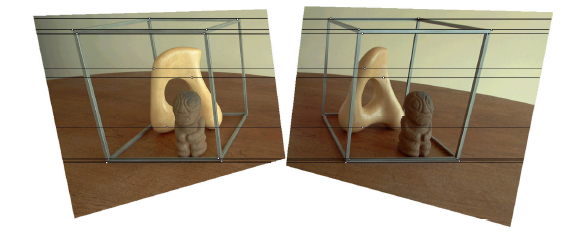
\includegraphics[width=1.\linewidth]{images/rectifiziertesBildAusZZ.png}
 	\captionof{figure}{Beipiel eines rektifizierten Bildes. Quelle: \cite{ZZ}} 
 \end{minipage}\\ \\

 \begin{minipage}{\linewidth}
	\centering
	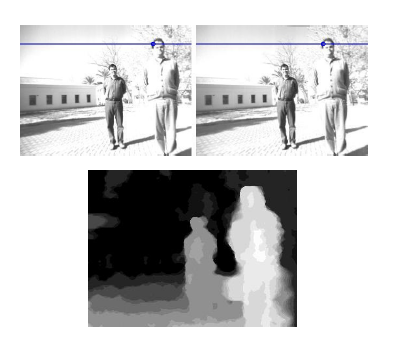
\includegraphics[width=1.\linewidth]{images/Disparity.png}
	\captionof{figure}{Beispiel einer einfachen Tiefenkarte eines Stereobildpaares nach der Rektifizierung. Quelle: \cite{Javier}} 
\end{minipage}\\ \\
 
Die Rektifizierung, allem voraus vor allem die Optimierung des Rektifizierungvorgangs, von Stereo- oder auch mulitplen- Kamerasystemen, wird heutzutage von vielen Entwicklergruppen der Computer Vision untersucht(Der satz ist mist!). Es gibt mittlerweile viele Ansätze, jedoch funktionieren nicht alle bei den selben Fällen. So setzten zum Beispiel manche Rektifizerungsalgorithmen voraus, dass die Bilder von Kameras mit selber Auflösung aufgenommen wurden. Ein Beispiel ist die Rektifizierung welche in \textit{Matlab} verwendet wird \cite{MatlabRec}. Die Rektifizierung wurde anhand einer Methode implementiert, welcher sich ähnlich verhält wie in \cite{FusielloSite} beschrieben. Die Grundidee hier hinter ist, dass die Kameramatrizen von zwei Kameras so aufgebaut sind dass die intrinsischen Parameter die selben sind, sie sich aber in ihren Rotationen und Translationen voneinander unterscheiden. Die extrinsischen Kameraparameter werden dann dementsprechend so manipuliert, dass die Bildebenen Achsenparallel zueinander stehen\cite{FusielloSite,Fusiello}. Um horizontale Epipolarlinien zu erhalten muss gleichzeitig die Basislinie zwischen den zwei Kamerazentren parallel zur neuen x-Achse beider Kameras sein. Zudem soll, um eine angemessene Rektifizierung zu gewährleisten, müssen konjugierende Punkte die selbe vertikale Koordinate haben. Dies wird hier durch die die Bedingung gewährleistet, dass beide Kameras die selben intrinsischen Parameter haben\cite{FusielloSite}. Eine Frage welche mit unter in dieser Arbeit beantwortet werden sollte, war, ob es möglich ist, ohne deutlich größeren Aufwand eine Kamerakalibrierung und Szenerekonstruktion mit Kameras unterschiedlicher Auflösung zu gewährleisten. Im Kapitel (KAPITELLINK EINFÜGEN), in welchem ausführlich die Epipolargeometrie vorgestellt wurde, wurde bereits bezug auf die unterschiedlichen Auflösungen genommen. Prinzipiell spielen unterschiedliche intrinsische Kameraparameter keine Rolle, wenn es um die Rekonstruktion der Kameraposen geht, da die Fundamental Matrix und die essentielle Matrix die Information über die intrinsischen und extrinsischen Kameraparameter besitzen und es klar gestellt wurde, dass die Bildkoordinatensysteme der Kameras nicht identisch sein müssen. \cite{Elements}. In dieser Arbeit wurde ein Rektifizierungsalgorithmus nach \textit{Zhang}\cite{ZZ} implementiert, welcher sich die Fundamentalmatrix zu nutzen macht. \textit{Loop} und \textit{Zhang} zerlegen jede Kollinearität in eine Ähnlichkeitstransformation, eine Schertransformation und eine projektive Transformation. Die projektive Komponenten wird dabei in einem nichtlinearen Optimierungsprozess so affin wie möglich gemacht.\cite{Fusiello,ZZ}. Im folgenden wird zunächst der genaue Vorgang des implementierten Algorithmus genauer erklärt und 
\textcolor{red}{des Weiteren werden zwei Beispiele vorgestellt, welche die Bilder des Minimalbeispiels einmal mit gleichen intrinsischen Parametern und einmal mit unterschiedlichen intrinsischen Parametern der Kamera aufzeigt. Es wird sich Herausstellen, dass beide Beispiele eine gelungene Rektifizierung der Bilder aufweisen.(Nochmal genau nachprüfen ob das geht!!!)}\\

Während sich einige Rektifizierungsverfahren im 3D-Raum abspielen, wird beim Verfahren nach \textit{Zhang}, hauptsächlich im 2D-Raum gearbeitet. Des Weiteren wird vorausgesetzt, dass die Fundamental Matrix \textit{F} und somot auch korrespondierende Punkte bereits bekannt sind. Sind die intrinsischen Kameraparameter bekannt, so wird aus der Fundamentalmatrix die Essentielle Matrix. Das Verfahren kann sowohl in einem kalibrierten als auch in einen unkalibrierten Fall angewendet werden\cite{ZZ}. Im Algorithmus wurde der unkalibrierte Fall implementiert und somit wird in der Erläuterung und in den danach folgenden Beispielen die Fundamentalmatrix \textit{F} verwendet. Die korrespondierenden Punkte werden mit \textit{x} für das erste beziehungsweise \textit{x'} für das zweite Bild definiert, die Kamerazentren dementsprechend mit \textit{C} und \textit{C'}. Bildebene der ersten Kamera wird mit \textit{I} definiert und die Bildebene von Kamera zwei mit \textit{I'}, die entsprechenden Epipole mit \textit{e} und \textit{e'}. Der Prozess der im Algorithmus erfolgt kann quasi als eine Transformation der Epipolar Geometrie eines Bildpaares in eine kanonische Form angesehen werden. Diese Transformation wird durch eine Homographiematrix durchgeführt, welche sich aus den bereits erwähnten drei Komponenten zusammenstellt. Zu Beginn sei noch erwähnt dass wir pro Bild zwei unterschiedliche Homographien \ensuremath{H} und \ensuremath{H'} brauchen. Die Fundamentalmatrix liefert, die Epipolarbedingung, dass $x'^TFx=0$ ergibt, wenn $x'$ auf der zu $x$ korrespondierenden Epipolarlinie liegt. Die korrespondierenden Punkte $x$ und $x'$ werden, für die Rektifizierung, jeweils mit den Homographien $H$ und $H'$ verrechnet.

\begin{gather}
	\bar{x}= Hx\\
	\bar{x'}= Hx'
\end{gather}\\

Die Fundamentalmatrix, welche sich aus durch die Rektifizierten korrespondierenden Punkte resultiert, wird mit $\bar{F}$ bezeichnet. Daraus folgt für die Fundamentalmatrix folgendes:

\begin{gather}
	\bar{x'}^T\bar{F}\bar{x} = 0\\
	\leadsto x'^TH'T\bar{F}Hx=0\\
	\leadsto F = H'^T[i]_xH
\end{gather}\\

Das Ziel ist es diese zwei Homographien in deren bereits erwähnten projektiven und affinen Komponenten zu zersetzten, wobei diese die jeweils entstehenden Bildverzerrungen minimieren sollen. Die Homographiematrizen bestehen aus drei Linien, welche jeweils durch den Epipol verlaufen. Des Weiteren werden noch ein paar weitere Bedingungen für die jeweils drei Linien festgelegt. So müssen die Linien $v$ und $v'$ sowie $w$ und $w'$ korrespondierende Epipolarlinien sein. Diese Bedingung schafft eine geometrische Verbindung beider Bilder zueinander und ist gerade bei der Minimierung der durch die Rektifizierung entstehenden Bildverzerrung von Bedeutung.

\begin{gather}
H = \begin{bmatrix}
u^T\\v^T\\w^T
\end{bmatrix} =
\begin{bmatrix}
u_a&u_b&u_c\\
v_a&v_b&v_c\\
w_a&w_b&w_c
\end{bmatrix}\\
H' = \begin{bmatrix}
u'^T\\v'^T\\w'^T
\end{bmatrix} =
\begin{bmatrix}
u'_a&u'_b&u'_c\\
v'_a&v'_b&v'_c\\
w'_a&w'_b&w'_c
\end{bmatrix}	
\end{gather}\\

Für die Bestimmung der einzelnen Komponenten von $H$ und $H'$ werden diese in ihre projektiven und affinen Teilstücke zerlegt. Davor wird noch die letzte Komponente $w_c$ raus dividiert, um somit  skaleninvariante Matrizen $H$ und $H'$ zu bekommen. 

\begin{gather}
H = \begin{bmatrix}
u^T\\v^T\\w^T
\end{bmatrix} =
\begin{bmatrix}
u_a&u_b&u_c\\
v_a&v_b&v_c\\
w_a&w_b&1
\end{bmatrix}\\
H' = \begin{bmatrix}
u'^T\\v'^T\\w'^T
\end{bmatrix} =
\begin{bmatrix}
u'_a&u'_b&u'_c\\
v'_a&v'_b&v'_c\\
w'_a&w'_b&1
\end{bmatrix}	
\end{gather}\\

Beide Matrizen werden nun auf die selbe Weise in ihre projektiven und affinen Bestandteile zerlegt.

\begin{gather}
	H = H_p \cdot H_a\\
	H' = H'_p \cdot H'_a
\end{gather}\\

$H_p$ ist die projektive Komponente, sie bezieht sich nur auf die letzte Zeile der Matrix $H$ und wirkt sich somit auch nur auf die homogene Komponenten der mit ihr verrechneten Punkte aus. 

\begin{gather}
	H_p = 
	\begin{bmatrix}
		1&0&0\\
		0&0&1\\
		w_a&w_b&1
	\end{bmatrix}
\end{gather}\\

Die affine Komponeten $H_a$ lässt sich aus $H$ und $H_p$ konstruieren. Es gilt:

\begin{gather}
	H_a= H \cdot H^{-1}_p = 
	\begin{bmatrix}
	u_a-v_cw_b&v_cw_a-v_a&0\\
	v_a-v_cw_a&v_b-v_cw_b&v_c\\
	0&0&1
	\end{bmatrix}
\end{gather}

Für die Matrizen $H_p'$ und $H_a'$ gilt das selbe nur mit den Epipolarlinien $u'$, $v'$ und $w'$.
Die projektive Matrix sogt dafür, dass die Epipole beider Bilder ins unendliche gesetzt werden und die Epipolarlinien der Bilder jeweils parallel zueinander verlaufen. Zu Beginn wurde erwähnt dass es eine Zerlegung in eine projektive, eine Ähnlichkeits- und eine Scherungstransformation gibt. Die projektive Komponente ist mit $H_p$ und $H_p'$ bereits vollständig definiert. Was nun noch fehlt ist die Zerlegung der affinen Matrizen $H_a$ und $H_a'$ in ihre jeweiligen Ähnlichkeits- und Scherungstransformationen. 

\begin{gather}
	H_a = H_s \cdot H_r\\
	H_r = 
	\begin{bmatrix}
	v_b-v_cw_b&	v_a-v_cw_a&0\\
	v_a-v_cw_a&v_b-v_cw_b&v_c\\
	0&0&1
	\end{bmatrix}\\
	H_s = 
	\begin{bmatrix}
	u_a&u_b&u_c\\
	0&1&0\\
	0&0&1
	\end{bmatrix}
\end{gather}\\

$H_r$ und auch $H_r'$ definieren eine Rotation und auch eine Verschiebung, welche die bereits parallelen Epipolarlinien beider Bilder zueinander parallel und horizontal ausrichtet. Durch die Verschiebung werden die korrespondierenden Epipolarlinien noch auf die selbe Höhe verschoben. Somit entstehen die gewünschten Scanlinien in den Bildern. Die Matrix $H_s$ und $H_s'$ wirken sich nur auf die $u$-Elemente der Matrix $H$ und $H'$ aus und definieren eine Scherung. Sie haben keine Auswirkung auf die Rektifizierung an sich aber sorgen dafür, dass die horizontale Verzerrung der beiden Bilder zueinander reduziert wird.\\

\subsection{Projektive Transformation}

Die projektiven Matrizen $H_p$ und $H_p'$ werden von den Linien $w$ und $w'$ bestimmt. $w$ und $w'$ sind dabei jedoch nicht unabhängig. Definiert werden sie durch einen Punkt $z = \begin{bmatrix}
\lambda&\mu&0\end{bmatrix}^T$, welche die, durch die Rektifizierung entstehende, Bildverzerrung minimieren soll. Für beide Bilder werden $w$ und $w'$ folgendermaßen gewählt

\begin{gather}
	w = [e]_x \cdot z\\
	w'= F\cdot z
\end{gather}\\

Jedes beliebige $z$ würde zwei korrespondierende Epipolarlinien definieren, um ein $z$ zu finden, welches die Verzerrung der Bilder minimiert, wird ein Kriterium aufgestellt, welches ein $z$ finden soll, dass die Verzerrung minimal halten wird. Minimierung bedeutet in diesem Falle, dass versucht wird die Matrizen $H_p$ und $H_p'$ so affin wie möglich zu machen. So affin wie möglich bedeute, dass die Werte von $w_a$ und $w_b$ so nah wie möglich an den Wert 0 gebracht werden sollen.

\begin{gather}
	H_p = 	\begin{bmatrix}
	1&0&0\\
	0&0&1\\
	w_a&w_b&1
	\end{bmatrix}
\end{gather}

Jedoch sollen sie nicht ganz null werden, da die projektive Matrix dann keine projektive mehr wäre, sondern eine affine.  Deswegen heißt es auch sie soll so affin wie möglich gemacht werden. Das selbe gilt natürlich auch für $w_a'$ und $w_b'$ aus $H_p'$. Wäre das der Fall, so wären die beiden Epipole $e$ und $e'$ bereits im unendlichen und die Matrizen $H_p$ und $H_p'$ hätten keine Auswirkungen auf die Punkte. Für die Minimierung wird die Methode des \textit{least-square-fitting}, also die Anpassung des kleinsten Quadrats, genutzt\cite{leastSquare}. Es werden also die Gewichtungen der Punkte in beiden Bildern in der Methode der Anpassung der kleinsten Quadrate verbaut, welche versucht eine Funktion zu finden, die einen Wert für $z$ berechnen soll welcher die Bildverzerrung minimal hält. \textcolor{red}{Anders ausgedrückt man sucht einen Wert für $z$, welcher am nächsten an den gegebenen Punktesammlungen der jeweiligen Bildern dran liegt, wobei für $z$ bereits gilt, dass es sich um einen Punkt im Unendlichen handeln soll}\cite{ZZ,leastSquare}. Angenommenem, dass die Annäherungsfunktion $g(x)$ eine Funktion $f(x)$, mit $x \in [a,b]$, annähern soll, dann versucht die Methode, die Summe der Quadrate der oridnatischen Differenzen, welche zwischen den von der Funktion generierten Punkten und den Punkten aus den Daten gewonnen wird, zu minimieren\cite{leastSquare,Margulies.}. Zum Beispiel werden $n$ Datenpunkte angenommen, dann gilt:

\begin{gather}
	e = \sum_{i=1}^{n}[f(x_i)-g(x_i)]^2
\end{gather}

Für die Minimierung der Bildverzerrung werden die Gewichtungen der Punkte beider Bilder benötigt. $p_i$ beinhaltet alle Punkte von Bild eins und $p_j$ beinhaltet alle Punkte von Bild zwei. Angenommen wir nehmen einen Punkt aus Bild eins $p_{i1} = \begin{bmatrix}p_{i1,u}&p_{i1,v}&1\end{bmatrix}^T$, so soll dieser Punkt mit der Matrix $H_p$ zu einem Punkt der Form  $p_{i1} = \begin{bmatrix}\frac{p_{i1,u}}{w_i}&\frac{p_{i1,v}}{w_i}&1\end{bmatrix}^T$ transformiert werden. $w_i$ ist die Gewichtung welche durch die Verrechnung von $w$ mit $p_i$ zustande kommt.

\begin{gather}
	w_i=w^Tp_i
\end{gather} 

Ist die Gewichtung der Punkte identisch gibt es keine projektive Verzerrung und die Homographie ist eine affine Transformation. Jedoch wenn die Epipole der Bilder ins Unendliche transformiert werden sollen, so können $H_p$ und $H_p'$ keine affine Homograhien sein. Sonst könnte man die Epipole nur innerhalb der affinen Ebenen, sprich den Bildebenen, verschieben. Also bildet der Versuch $H_p$ und $H_p'$ so affin wie möglich zu machen die Basis für die Minimierung. Im Realbeispiel werden alle Pixel des Bildes verwendet. Die Rektifizierung wurde im aufgeführten Beispiel anhand des erstellten Minimalbeispiels durchgeführt, somit wurden die Eckpunkte des Quaders des jeweiligen Bildes für die das Minimierungskriterium verwendet. Es wird eine Funktion nach dem Prinzip der Anpassung der kleinsten Quadrate aufgestellt, welche die Abweichung der Gewichtung der Punkte in Bezug auf die Gewichtung des Bildzentrums $p_c$ berechnet.$p_c$ ergibt sich aus der Mittelung aller verwendeten Punkte eines Bildes $p_c = \frac{1}{n} \sum_{i=1}^{n} p_i$, dessen Gewichtung ergibt sich aus $w_c= w^T p_c$. Die gesuchte Abweichung ausgedrückt in der Anpassung der kleinsten Quadreate ergibt dann die folgende Formel.\\

\begin{gather}
	\sum_{i-1}^{n}\Big[\frac{w_i-w_c}{w_c} \Big]^2\\
	\leadsto \sum_{i=1}^{n}\Big[\frac{w^T (p_i-p_c)}{w^Tp_c} \Big]^2
	\leadsto \sum_{i=1}^{n}\Big[\frac{w^T (p_i-p_c)(p_i-p_c)^Tw}{w^Tp_cp_c^Tw} \Big]
\end{gather}\\

Vereinfacht lässt sich das auch in einer Matrixgleichung angeben

\begin{gather}
	\frac{w^TPP^Tw}{w^Tp_cp_c^Tw}
\end{gather}

in welcher für $P$ gilt:

\begin{gather}
	P=\begin{bmatrix}
	p_{1,u}-p_{c,u}&p_{2,u}-p_{c,u}&...&p_{i,u}-p_{c,u}\\
	p_{1,v}-p_{c,v}&p_{2,v}-p_{c,v}&...&p_{i,v}-p_{c,v}\\
	0&0&...&0	
	\end{bmatrix}
\end{gather}

die Gleichungen 4.79 bis 4.83 werden ebenfalls für die Punkte $p_j$ in Bild zwei aufgestellt. So ergibt sich für das zweite Bild die Matrixgleichung:

\begin{gather}
	\frac{w'^TP'P'^Tw'}{w'^Tp_c'p_c'^Tw'}
\end{gather} 

Das Ziel ist es einen Wert für $z$ zu finden, welches bis jetzt noch nicht ersichtlich in den Gleichungen vorkommt. Also werden $w$ und $w^T$ noch mit ihren Definitionen aus den Gleichungen 4.75 und 4.76 ersetzt. Gleichzeitig werden die Gleichungen 4.82 und 4.84 summiert um die Gleichung zu erhalten, welche sich auf beide Bilder gleichzeitig bezieht und somit eine Lösung für $z$, das für beide Bilder gilt, gesucht werden kann.

\begin{gather}
	\frac{z^T[e]_x^TPP^T[e]_xz}{z^T[e]_x^Tp_cp_c^T[e]_xz}+\frac{z^TF^TP'P'^TFz}{z^TF^Tp_c'p_c'^TFz}
\end{gather}

Für den weiteren Verlauf werden die Ausdrücke noch durch die Variablen $A,B,A'$ und $B'$ vereinfacht.

\begin{gather}
	A = [e]_x^TPP^T[e]_x\\
	B=[e]_x^Tp_cp_c^T[e]_x\\
	A'=F^TP'P'^TF\\
	B'= F^Tp_c'p_c'^TF\\
	\leadsto 
	\frac{z^TAz}{z^TBz}+\frac{z^TA'z}{z^TB'Fz}
\end{gather}\\

Da die dritte Komponente von $z$ laut definition null sein soll, wird zu $z = \begin{pmatrix}
\lambda\\ \mu\end{pmatrix}$ umgeschrieben. $A,B,A'$ und $B'$ sind 3x3-Matrizen, von welchen uns dann nur noch der erste 2x2-Block interessiert. Bei dem somit aufgestellten Minimalisierungs Kriterium, handelt es sich um ein nicht lineares optimierungs Problem. Die Gleichung 4.90 ist dann minimiert, wenn die erste Ableitung dieser Funktion nach $\lambda$ = gleich null ist. Es entsteht also ein Polynom mit dem Grad sieben, da die 4.90 die Summe zweier rationaler Funktionen ist, welche jeweil das Verhältnis von quadratischen Polynomen darstellt.

\begin{gather}
\textit{Hier soll das Polynom aufgestllt werden, ist aber nicht mehr klar wie das ging!!!}
\end{gather}\\

Für die nicht lineare Optimierung wird das gesamte Polynom aufgeteilt, so minimieren wir zunächst $\frac{z^TAz}{z^TBz}$ und danach $\frac{z^TA'z}{z^TB'z}$. So entstehen für $z$ zunächst zwei Lösungen 
$\hat{z_1}$ und $\hat{z_2}$, welche über eine Mittelung eine ersten Schätzung für $z$ geben, welche schon ziemlich nah an den optimalen Wert heranreicht.

\begin{gather}
	z = \frac{\frac{\hat{z_1}}{\| z_1 \|}+\frac{\hat{z_2}}{\| z_2 \|}}{2}
\end{gather}\\

Da es sich um eine nicht lineare Optimierung handelt ist die Minimierung von  $\frac{z^TAz}{z^TBz}$ gleichzusetzen mit der Maximierung von  $\frac{z^TBz}{z^TAz}$. Beide als eine Funktion von $f(z)$. Matrix $A$ wird mit der Choleskyzerlegung in zwei höhere Dreiecksmatrizen zerlegt $A = D^TD$\cite{Fortran77}. Dies geht nur da $A$ nachweislich eine symmetrische und positiv-definite Matrix ist.\cite{Fortran77} positiv-Definite bedeutet, dass die Singulärwerte von $A$ immer positiv bleiben, egal mit welchem Vektor $z$ diese multipliziert wird. \textcolor{red}{(HIER NOCH LITERATUR FINDEN UND NOCHMAL PRÜFEN OB DEFINITION SO STIMMT)}.  Des Weiteren wir definiert, dass $y = Dz$ ist und $f(z)$ wird dann zu einen $\hat{f}(y)$

\begin{gather}
	A = D^TD\\
	y= Dz \leadsto z= D^{-1}y\\
	f(z)= \frac{z^TBz}{z^TAz}\\
	\leadsto 
	f(z)=\frac{z^TBz}{z^TD^TDz}\\
	\hat{f}(y)= \frac{y^TD^{-T}BD^{-1}y}{y^Ty}
\end{gather}

Durch die Defintion von $y = Dz$ ist $y$ bis auf einen Skalierungsfaktor definiert. $\hat{f}(y)$ ist maximiert, wenn $y$ gleich dem Eigenvektor von $D^-TBD-1$ ist, welcher mit dem größten Eigenwert assoziert wird. Zum Schluss erhalten wir dann einen Wert für $\hat{z_1}$ mit $\hat{z_1} = D^{-1}y$. Exakt das selbe Verfahren wird für die Findung von $z_2$ mit  $\frac{z^TB'z}{z^TA'z}$ angewandt. \textcolor{red}{Sind $z_1, z_2$ und eine erste Schätzung für $z$ gefunden, so kann ein Wert für $z$ gesucht werden, welcher noch näher an ein optimales Ergebnis heranreicht. Beide Lösungen $z_1$ und $z_2$, werden in die Funktion $f(z)$ eingesetzt und es jeweils ein wert ermittelt, welcher am nächsten an einem Nullpunkt sich befindet. So kann iterativ eine optimale Lösung für $z$ gefunden werden.} Ist der Wert für $z$ bestimmt, so kann dieser die Gleichungen 4.75 und 4.76 eingesetzt werden und $w$ beziehungsweise $w'$ bestimmt werden, welche die Elemente für die Matritzen $H_p$ und $H_p'$ bereitstellen.
Abbildung 4.7 zeigt in rot den Quader des Minimalbeispiels wie er in Kamera zwei abgebildet ist und in grün wie er in Kamera eins abgebildet ist. Kamera zwei ist horizontal zu Kamera eins verschoben und um $45\circ$ zu Kamera eins um die eigene vertikale Achse ein gedreht. Die Auflösungen beider Kameras sind identisch, sprich die intrinsischen Kameraparameter sind die selben. Abbildung 4.8 zeigt die momentanen Epipolarlinien. Die Epipolarlinien von Bild eins, also dem grünen Abbild, sind bereits Parallel, was aber keine Voraussetzung für die Funktion des Rektifizierungsalgorithmus ist. Der Schnittpunkt der Epipolarlinien von Bild zwei, also dem Roten Abbild, treffen sich in einem Punkt und bilden somit den Epipol von Bild zwei. 

\begin{minipage}{\linewidth}
	\centering
	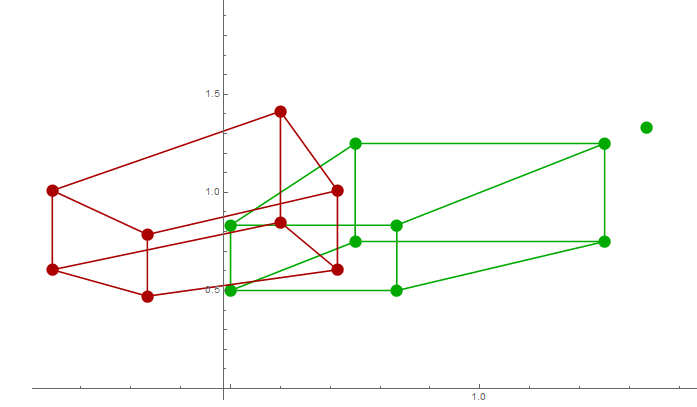
\includegraphics[width=.8\linewidth]{images/Rectification_one_same_Solutions.png}
	\captionof{figure}{Aufnahmen zweier Kameras mit den selben Auflösungen, Kamera eins(Grün) und Kamera(rot) zwei gelten jeweils \ensuremath{\zeta =1}} 
\end{minipage}\\ 

\begin{minipage}{\linewidth}
	\centering
	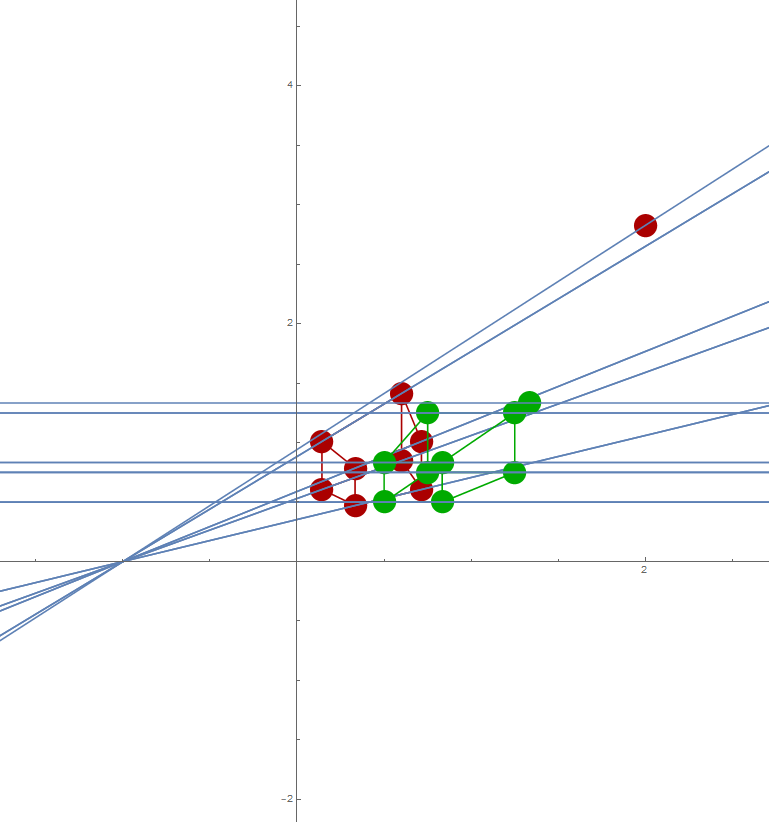
\includegraphics[width=.8\linewidth]{images/Rectification_two_same_Solutions.png}
	\captionof{figure}{Epipole für Kamera eins und Kamera zwei vor der Rektifizierung } 
\end{minipage}\\

\pagebreak

Werden nun die Matritzen $H_p$ und $H_p'$ auf die jeweiligen Punkte der Bilder, $p_i$ für Bild eins und $p_j$ für Bild zwei, angewandt, so kann man eine erste Veränderung beobachten. Abbildung 4.9 zeigt beide Quader aus Abbildung 4.7 nachdem die jeweiligen Bildpunkte mit den projektiven Matrizen multipliziert wurden. Der Epipol in Bild eins bleibt natürlich wie zuvor im unendlichen, jedoch kann man erkennen, dass der rote Quader aus Bild zwei sich verändert hat. Sein Epipol wurde ins Unendliche transformiert und parallele Linien sind nun auch auf dem Bild parallel. Das die Epipolarlinien bereits horizontal parallel zur x-Achse verlaufen ist Zufall und ist nach der Anwendung der projektiven Matrizen auch noch nicht verlangt. Das Anpassen der Epipolarlinien, dazu gehört sie zunächst von beiden Bilder aus parallel zur x-Achse verlaufen zu lassen und dann noch sie so zueinander anzupassen, dass sie zu Scanlinien über beide Bilder verlaufen, verlgeiche Abbildung 4.12, folgt im nächsten Schritt. \\


\begin{minipage}{\linewidth}
	\centering
	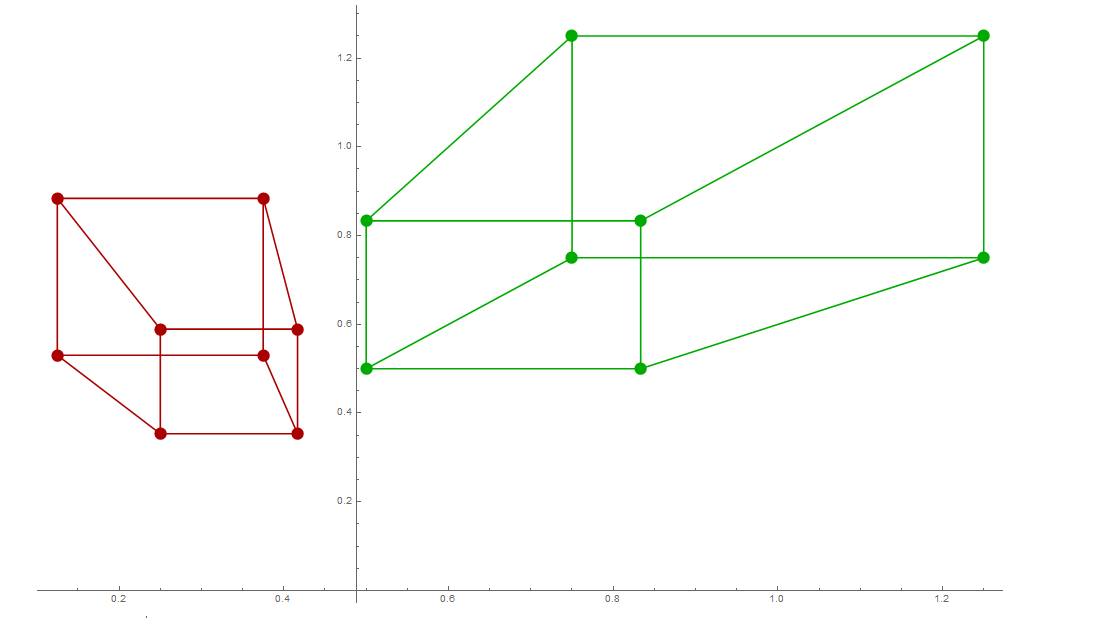
\includegraphics[width=1.\linewidth]{images/Rectification_Hp_same_Solutions.png}
	\captionof{figure}{Abbildung beider Bilder nach anwenden der Matrizen $H_p$ und $H_p'$. Die Epipole beider Bilder sind nun im unendlichen. Das die enstehenden parallelen Epipolarlinien auch hier schon horizontal ausgerichtet sind ist Zufall. Die Epipolarlinien sind immer parallel nach dieser Transformation aber die Richtung ist nicht immer automatisch bereits i = [1,0,0].} 
\end{minipage}\\ \\

\subsection{Ähnlichkeitstransformation}

Nachdem die Epipole ins Unendliche verschoben wurden, müssen diese nun so rotiert und verschoben werden, dass die Epipolarlinien als Richtung $i = \begin{bmatrix}1&0&0\end{bmatrix}$ haben und die Epipolarlinien beider Bilder zu einheitlichen Scanlinien werden. Für die Ähnlichkeitstransformation wird davon ausgegangen, dass $w$ und $w'$ bereits bekannt sind.$H_r$ und $H_r'$ wurden bereits aus der Zerlegung von $H_a$ und $H_a'$ gewonnen.

\begin{gather}
		H_r = 
	\begin{bmatrix}
	v_b-v_cw_b&	v_a-v_cw_a&0\\
	v_a-v_cw_a&v_b-v_cw_b&v_c\\
	0&0&1
	\end{bmatrix}\\
		H_r' = 
	\begin{bmatrix}
	v_b'-v_c'w_b'&	v_a'-v_c'w_a'&0\\
	v_a'-v_c'w_a'&v_b'-v_c'w_b'&v_c'\\
	0&0&1
	\end{bmatrix}\\
\end{gather}

$w$ und $w'$ sind bereits bekannt, Mit Hilfe von $F$, können $v_a$ und $v_b$ ersetzt werden. Dazu kann die letzte Zeile von F nach $v_a, v_b$ und $v_c$ aufgelöst werden. Für $v_a', v_b'$ und $v_c'$ wird die letzte Spalte von F verwendet. So können folgende Gleichungen für $v_a, v_a',v_b, v_b', v_c$ und $v_c'$ gewonnen werden. 

\begin{gather}
	F = H'^T[i]_xH\\
	F=
	\begin{bmatrix}
	v_aw_a' - v_a'w_a&v_bw_a' - v_a'w_b&v_cw_a' - v_a'\\
	v_aw_b' - v_b'w_a&v_bw_b' - v_b'w_b&v_cw_b' - v_b'\\
	v_a - v_c'w_a&v_b - v_c'w_b&v_c-v_c'
	\end{bmatrix}\\
	v_a = F_{31}+v_c'w_a\\
	v_b = F_{32}+v_c'w_b\\
	v_c = F_{33}+v_c'\\
	v_a' = v_cw_a'-F_{13}\\
	v_b' = v_cw_b'-F_{23}\\
	v_c' = v_c -F_{33}
\end{gather}

Eingesetzt in die jeweiligen Matrizen $H_r$ und $H_r'$, entstehen die folgenden Matrizen in Gleichungen 4.114 und 4.115, welche nur noch die unbekannte $v_c'$ beinhalten. Die gemeinsame Variable $v_c'$ zeigt die geometrische Verbindung beider Bilder in ihrer Verschiebung entlang ihrer v-Richtung. Es wird also ein Offset von $F_33$ benötigt, um die Epipolarlinien horizontal zu Scanlinien auszurichten. \textcolor{red}{Den Wert für $v_c$ wird so ermittelt, dass das Minimum einer v-Koordinaten eines Pixel als minimum den Wert null besitzt }

\begin{gather}
	H_r = \begin{bmatrix}
	F_{32}-w_bF_{33}&w_aF_{33}-F_{31}&0\\
	F_{31}-w_aF_{33}&F_{32}-w_bF_{33}&F_{33}+v_c'\\
	0&0&1
	\end{bmatrix}\\
	H_r'=
	\begin{bmatrix}
	w_b'F_{33}-F_{23}&F_{13}-w_a'F_{33}&0\\
	w_a'F_{33}-F_{13}&w_b'F_{33}-F_{23}&v_c'\\
	0&0&1
	\end{bmatrix}
\end{gather}\\

Das Ergebnis der Bildpunkte $p_i$ und $p_j$ multipliziert mit den Matrizen $H_rH_p$ und $H_r'H_p'$ mit ist in Abbildung 4.10 zu sehen. Als letztes folgt noch die Scherungstransformation $H_s$ und $H_s'$ für die horizontale Entzerrung beider Bilder.\\ 

\begin{minipage}{\linewidth}
	\centering
	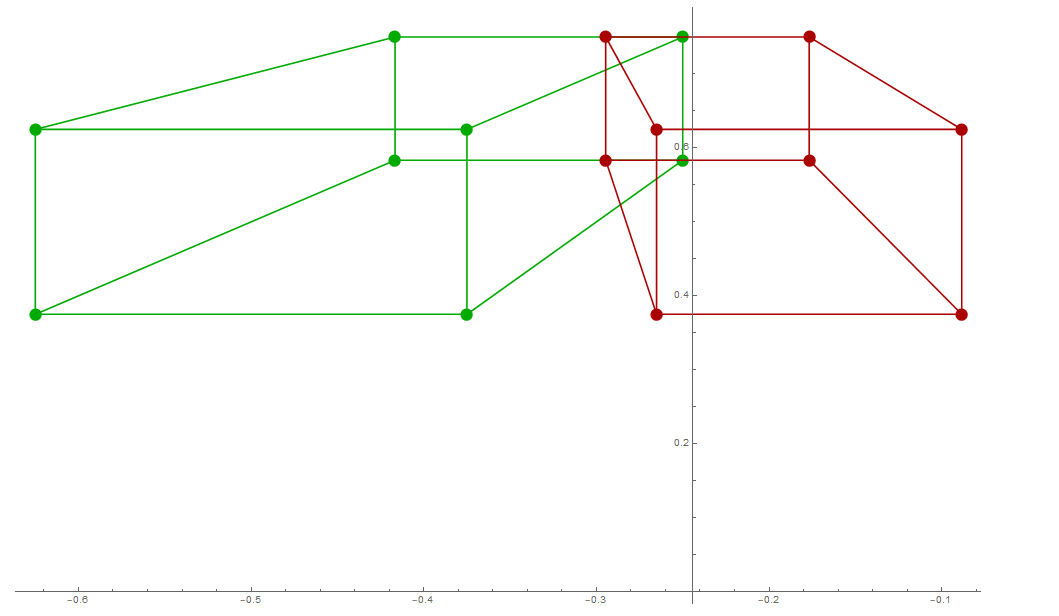
\includegraphics[width=1.\linewidth]{images/Rectification_HrHp_same_Solutions.png}
	\captionof{figure}{Abbildung beider Bilder nach anwenden der Matrizen $H_r \cdot H_p$ und $H_r' \cdot H_p'$. Die Epipolarlinien sind nun horizontal zueinander ausgerichtet} 
\end{minipage}\\ \\

\subsection{Scherungstransformation}

?????

\begin{minipage}{\linewidth}
	\centering
	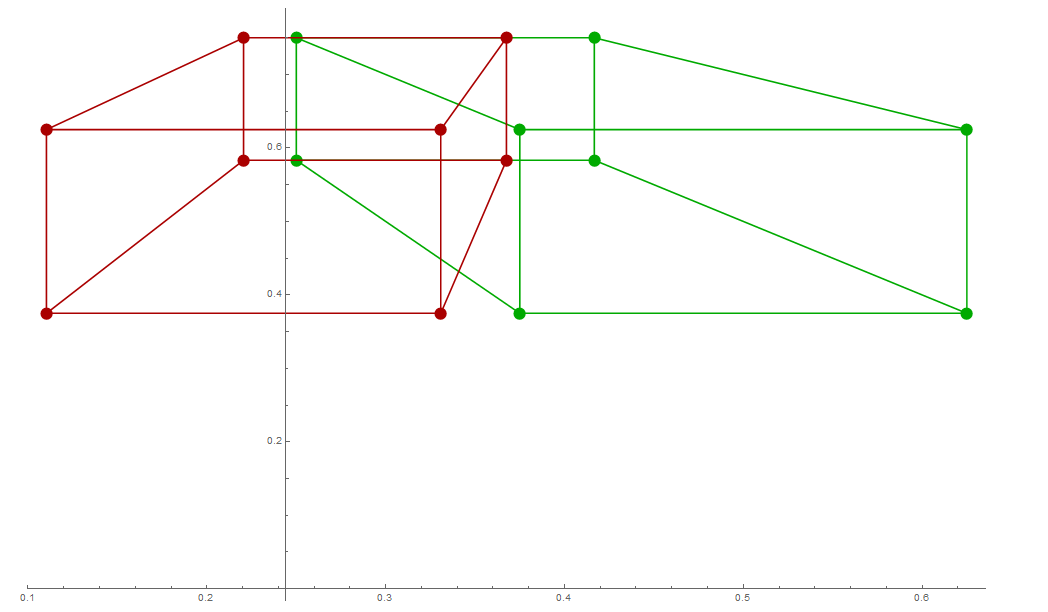
\includegraphics[width=1.\linewidth]{images/Rectification_HsHrHp_same_Solutions.png}
	\captionof{figure}{Abbildung beider Bilder nach anwenden der Matrizen $H_s \cdot H_r \cdot H_p$ und $H_s' \cdot H_r' \cdot H_p'$. Die horizontale Verzerrung wurde reduziert.} 
\end{minipage}\\ \\

\begin{minipage}{\linewidth}
	\centering
	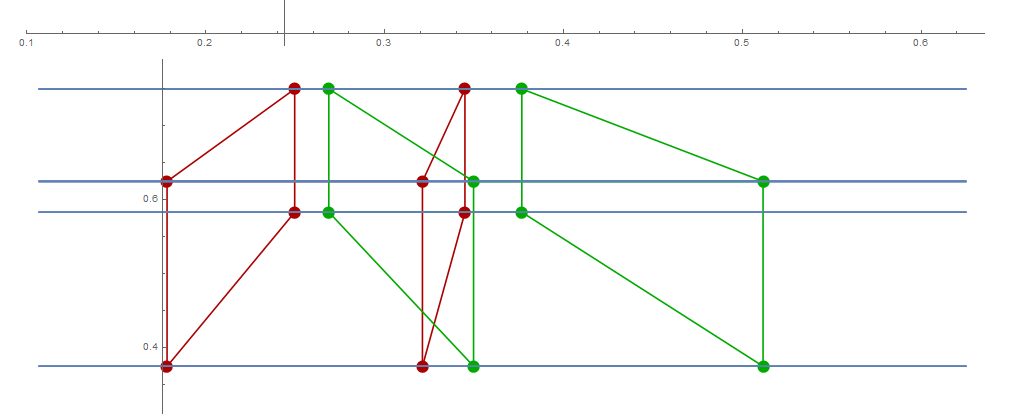
\includegraphics[width=1.\linewidth]{images/Rectification_four_same_Solutions.png}
	\captionof{figure}{In dieser Abbildung wurden die Epipolarlinien noch in den Grafikplot mit eingebaut} 
\end{minipage}\\ \\

%\begin{minipage}{\linewidth}
%	\centering
%	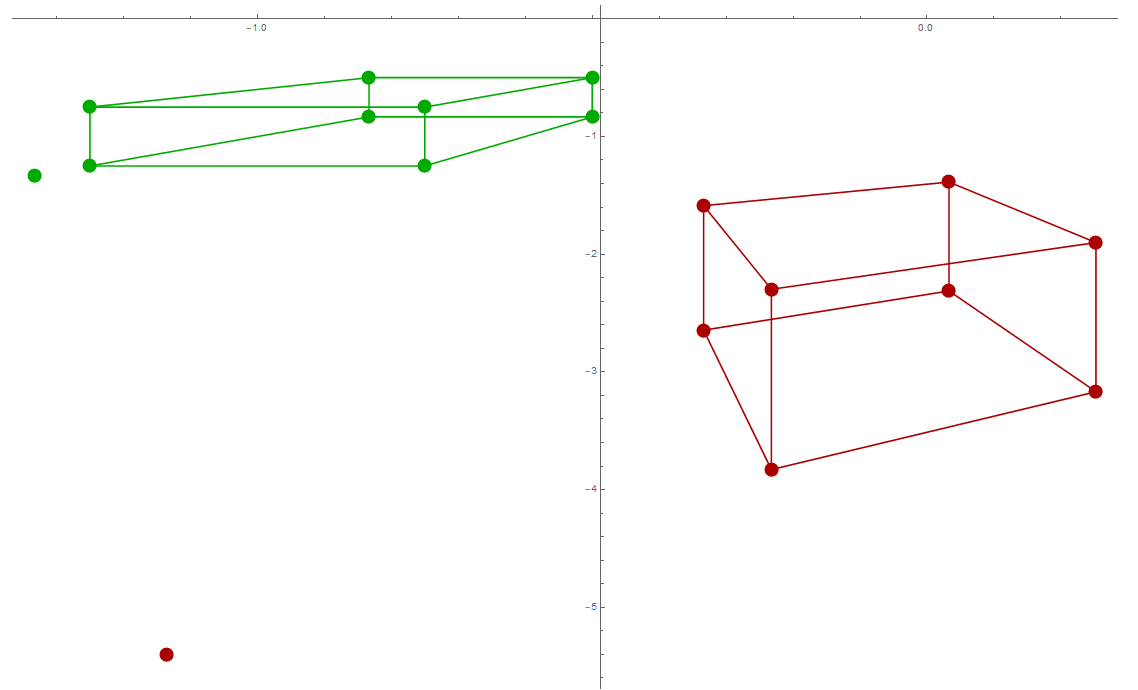
\includegraphics[width=1.\linewidth]{images/Rectification_one_different_Solutions.png}
%	\captionof{figure}{Aufnahmen zweier Kameras mit unterschiedlichen auflösungen, Kamera eins(Grün) besitzt für \ensuremath{\zeta} den Wert 1 und für Kamera zwei(rot) gilt jeweils \ensuremath{\zeta_x = 1.2} und \ensuremath{\zeta_y = 3.1}} 
%\end{minipage}\\ \\
%
%(Normalerweise in realbildern wird das bild bei unterschiedlicher Auflösung nicht verzerrt sondern nur "Vergrößert" oder zurecht "geschnitten". Dadruch dass beide Quader in einem Koordinatensystem verbaut wurden sieht das so aus)
%
%
%\begin{minipage}{\linewidth}
%	\centering
%	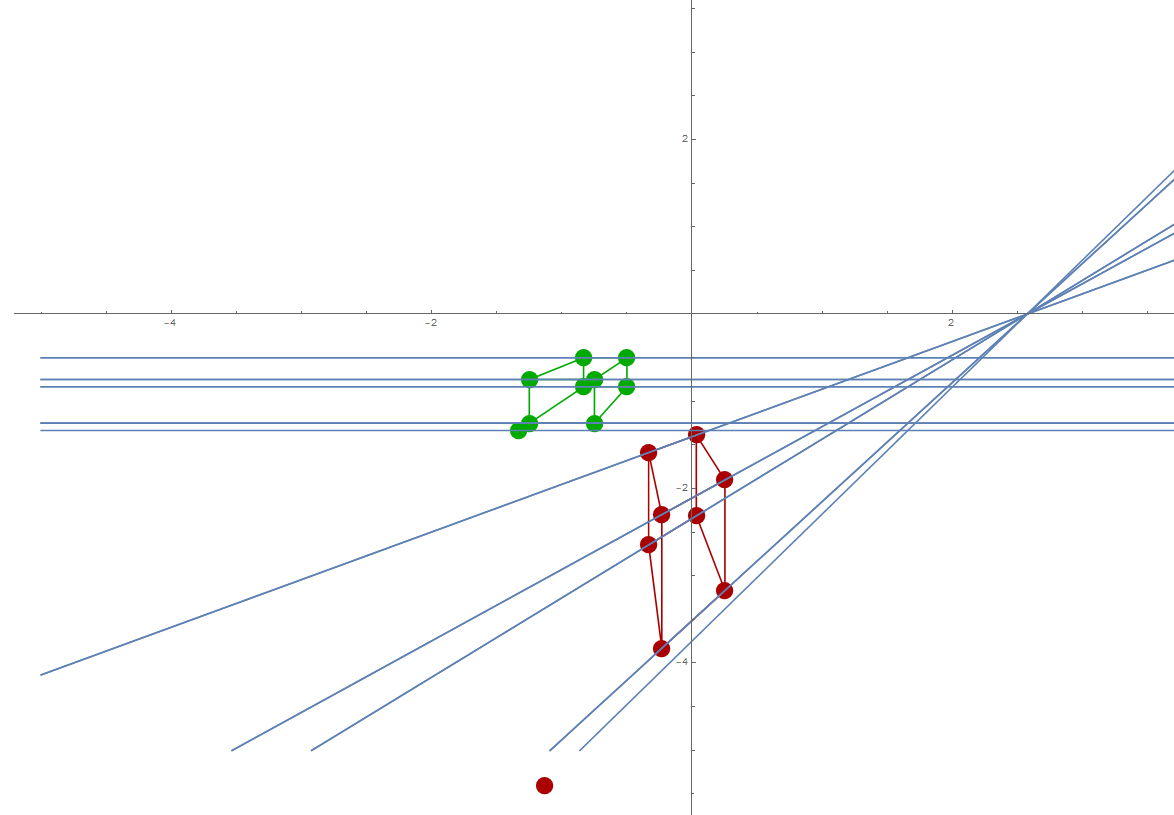
\includegraphics[width=1.\linewidth]{images/Rectification_two_different_Solutions.png}
%	\captionof{figure}{Epipole für Kamera eins und Kamera zwei vor der Rektifizierung } 
%\end{minipage}\\ \\
%
%
%\begin{minipage}{\linewidth}
%	\centering
%	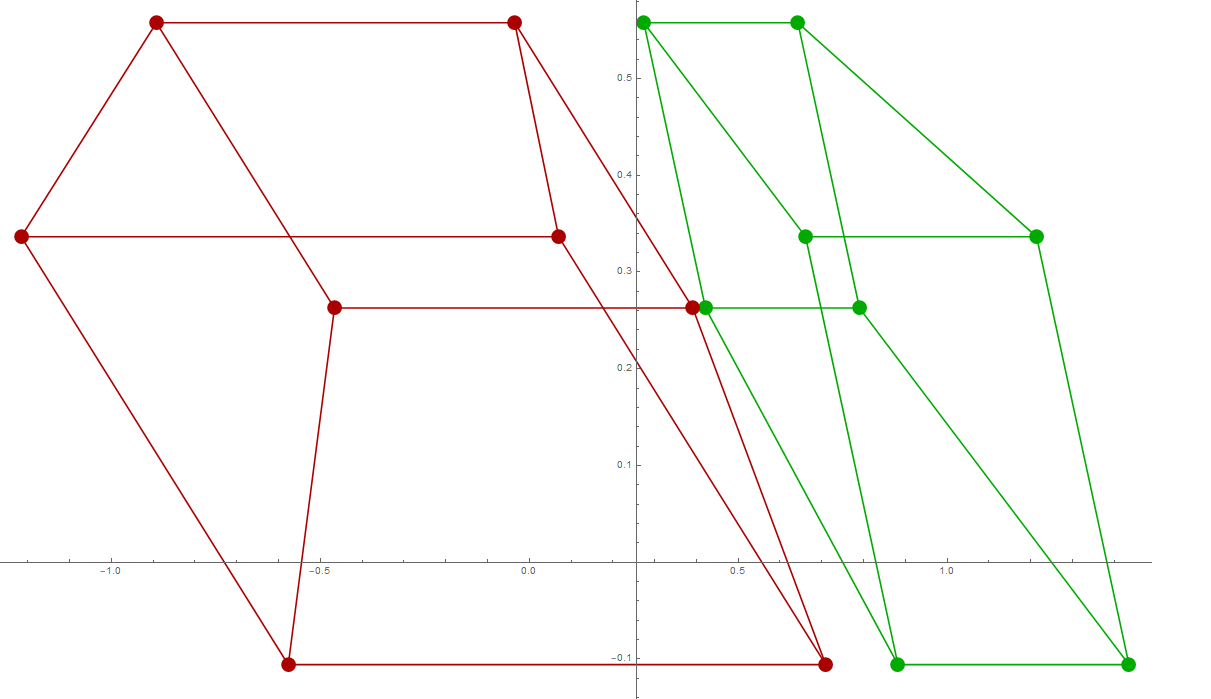
\includegraphics[width=1.\linewidth]{images/Rectification_three_different_Solutions.png}
%	\captionof{figure}{Nach dem die drei Homographien auf die Punkte angewandt sind die Eckpunkte des Quaders auf beiden Bilder auf den selben corresüondierenden Epipolarlinien} 
%\end{minipage}\\ \\
%
%
%\begin{minipage}{\linewidth}
%	\centering
%	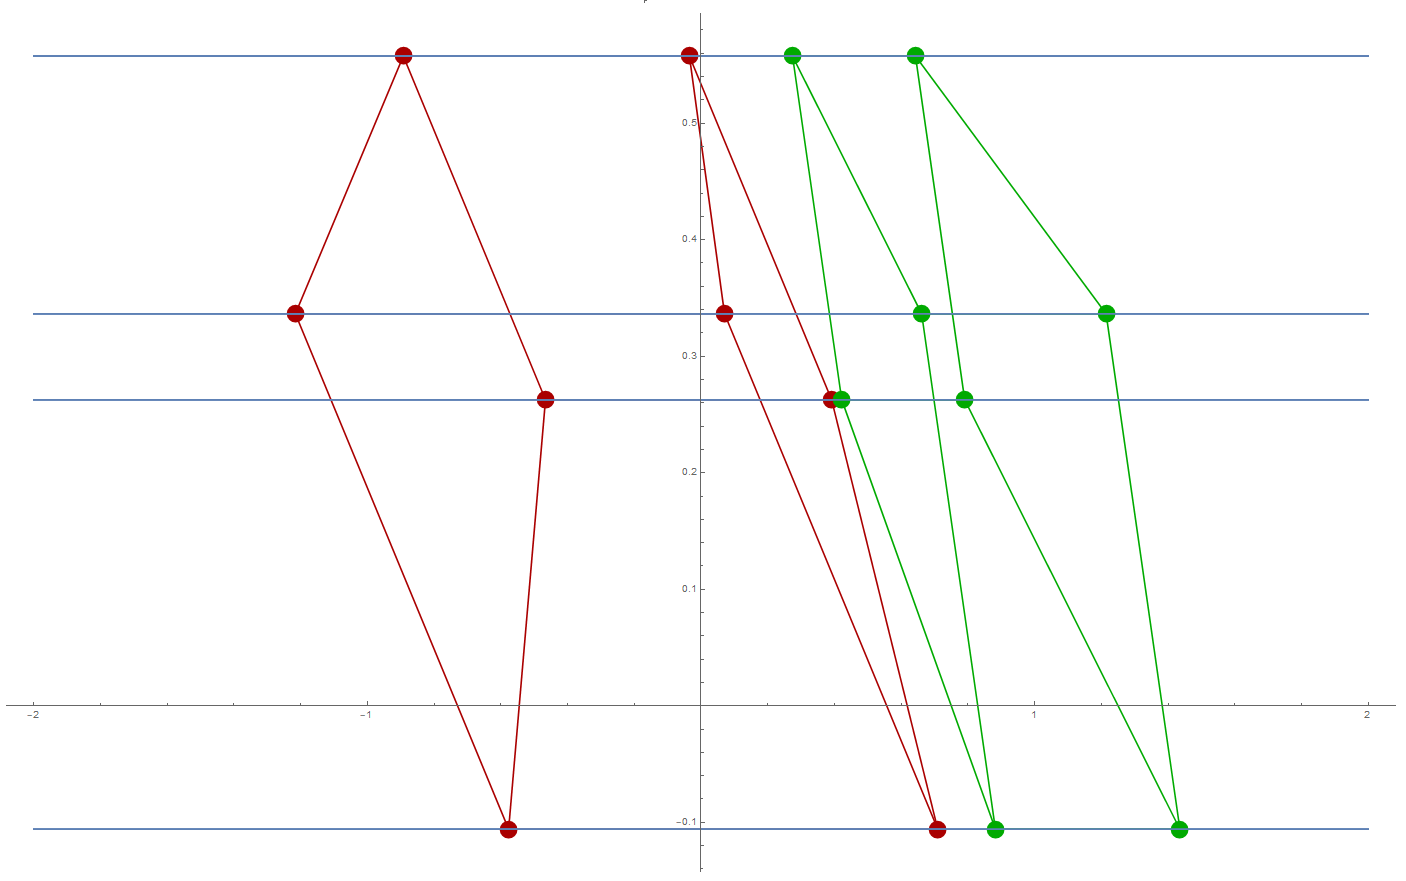
\includegraphics[width=1.\linewidth]{images/Rectification_four_different_Solutions.png}
%	\captionof{figure}{In dieser Abbildung wurden die Epipolarlinien noch in den Grafikplot mit eingebaut} 
%\end{minipage}\\ \\
